% Foveated Vision on a Moving Head: First Experiments
% VISGRAF Lab technical note. 12 November 2026.
% Build: pdflatex twice. Figures in figs/ come from the records of visgraf/foveal-motion (docs/runs/).
\documentclass[11pt,a4paper]{article}

\usepackage[T1]{fontenc}
\usepackage[utf8]{inputenc}
\IfFileExists{lmodern.sty}{\usepackage{lmodern}\usepackage{microtype}}{\usepackage[expansion=false]{microtype}}
\usepackage[a4paper,top=2.5cm,bottom=2.6cm,left=2.6cm,right=2.6cm]{geometry}
\usepackage{textcomp}
\usepackage{amsmath,amssymb}
\usepackage{booktabs}
\usepackage{tabularx}
\usepackage{array}
\usepackage{multirow}
\usepackage{xcolor}
\usepackage{enumitem}
\usepackage{graphicx}
\usepackage[font=small,labelfont=bf]{caption}
\usepackage{tikz}
\usetikzlibrary{arrows.meta,positioning,calc}
\usepackage{pgfplots}
\pgfplotsset{compat=1.16}
\usepgfplotslibrary{groupplots}
\usepackage[section]{placeins}
\usepackage[hidelinks]{hyperref}
\hypersetup{colorlinks=true,linkcolor=black!70!blue,citecolor=black!70!blue,urlcolor=black!70!blue,
  pdftitle={Foveated Vision on a Moving Head: First Experiments},
  pdfauthor={Luiz Velho, with Claude (Anthropic)},
  pdfsubject={VISGRAF technical note, 12 November 2026}}

% ---------------------------------------------------------------- VISGRAF cover
\IfFileExists{techrep-ic.sty}{%
  \usepackage{techrep-ic}%
  \newcommand{\MakeVisgrafCover}{%
    \TRNumber{15}   % <-- set the report number (printed as TR-26-XX)
    \TRYear{26}
    \TRMonth{11}
    \TRAuthor{Luiz Velho, Claude}
    \TRTitle{Foveated Vision on a Moving Head:\\First Experiments}
    \TRMakeCover}%
}{\newcommand{\MakeVisgrafCover}{}}

% ---------------------------------------------------------------- helpers
\newcommand{\code}[1]{\texttt{\small #1}}
\newcommand{\cell}{\raggedright\arraybackslash}
\newcolumntype{L}{>{\cell}X}
\setlist{itemsep=2pt,topsep=4pt}
\renewcommand{\arraystretch}{1.15}
\setlength{\emergencystretch}{1.5em}
\renewcommand{\topfraction}{0.9}\renewcommand{\bottomfraction}{0.6}\renewcommand{\textfraction}{0.08}\renewcommand{\floatpagefraction}{0.8}
\newcommand{\vb}[1]{\mathbf{#1}}
\newcommand{\emax}{e_{\max}}
% where a number comes from
\newcommand{\src}[1]{\textsuperscript{\,#1}}
\newcommand{\WS}{\src{W}}   % measured by Claude Code on the workstation
\newcommand{\SB}{\src{S}}   % measured in the Chat sandbox
\definecolor{cTarget}{HTML}{1F6FB4}
\definecolor{cAhead}{HTML}{D0602A}
\definecolor{cSide}{HTML}{2E8B57}

\title{\textbf{Foveated Vision on a Moving Head:\\First Experiments}}
\author{Luiz Velho\\[2pt] \normalsize with Claude (Anthropic)\\[2pt]
  \normalsize VISGRAF Lab, IMPA}
\date{\normalsize Technical Note \textperiodcentered{} 12 November 2026\\[2pt]
  \normalsize Software and records: \url{https://github.com/visgraf/foveal-motion}}

\begin{document}

\MakeVisgrafCover
\maketitle

\begin{abstract}
\noindent Our foveal vision experiments so far kept the head still: the eyes turned, the head did not move. This note
reports the first experiments in which it moves. A single foveated eye (log-polar, 2° fovea, 45° field) at the cyclopean
point walks straight down the Blender Classroom toward the board, 4.55\,m in steps of 10\,cm, rendered with
\emph{fov-render} through its new per-look head pose. Experiment M1 checks the motion end to end and measures the retinal
flow on the foveated raster under two gaze modes, fixating a target or looking ahead. Experiment M2 recovers range from
the head's own motion, triangulating each point between two looks with pixel-limited correspondence, and asks where in
the field that range is usable. Looking along the path, the fovea gets no usable range at any step up to 1\,m: its
finest pixels sit where there is no parallax. Fixating a point 22--47° off the heading, the fovea supports a range within
7.3\,\% (median) from a single 10\,cm step and 1.5\,\% from 0.5\,m. Under fixation, even a match with no measurable flow
carries range, relative to the fixated point; we therefore report the precision a match supports, not only the error
it happens to have. We also record what it took to get there: two preflight stops, two decisions and two corrected
readings.
\end{abstract}

\noindent\small Numbers carry their source: \WS\ measured by Claude Code on the RTX~4090 workstation (Blender 5.2.1,
OptiX) on the Classroom; \SB\ measured in the Chat sandbox (the \code{bpy} 5.2.1 wheel on CPU) on fov-render's
calibration room. Every number is in a record in the repository, \code{docs/runs/issue-1/} and \code{docs/runs/issue-3/},
or in the GitHub issue that reported it.\normalsize

% ================================================================================================
\section{Why move the head}\label{sec:why}

The active foveal playground~\cite{playground,tr11} explores a static scene from a fixed head: the eyes saccade, fixate,
triangulate what the fovea sees in stereo and decide where to look next. A fixed head limits what can be seen, but it
also hides one of the strongest cues an animal has: the flow of the retinal image when the head translates. For a static
point at range $\rho$, seen at an angle $\psi$ from the direction of travel, a step $T$ of the head moves its image by
about
\begin{equation}\label{eq:flow}
  \delta\theta \approx \frac{|T|\sin\psi}{\rho},
\end{equation}
zero at the focus of expansion ($\psi=0$) and largest broadside~\cite{lhp}. A foveated sensor samples the field very
unevenly: on our log-polar raster the pixel spacing grows linearly with eccentricity $e$,
$s(e)=s_0\,(1+e/E_2)$~\cite{schwartz,fovrendertr}. Where the eye points therefore decides which pixels see which flow.
Luiz's expectation, which this note starts to test, is that the foveated sensor helps under translation through that
flow.

fov-render~\cite{fovrender,fovrendertr} gained a moving head on 12 November 2026 (its issue \#20): a look may carry its own
head pose; without one it uses the scene's \code{EYE}. The server keeps no head state, and there is no body frame yet
(fov-render decisions D19, D20). The head moves between looks, never within one. With that, we opened a separate
repository, \code{visgraf/foveal-motion}~\cite{fm}, forked from the playground (its history kept, its code left as the
reference) and with fov-render pinned as a submodule. The decisions that shaped this first phase are in
Table~\ref{tab:decisions}.

\begin{table}[h]
\centering\small
\begin{tabularx}{\linewidth}{@{}lL@{}}
\toprule
M-D1 & An independent repository, \code{visgraf/foveal-motion}, carrying foveal-playground's history; fov-render as a submodule. \\
M-D2 & Monocular first: fov-render's cyclopean eye \code{C}, at the head origin, with the Foveated sensor. \\
M-D3 & The first test: the head walks straight from the back of the Classroom to the board. \\
M-D4 & Two gaze modes on the same path: fixating the board centre (\code{target}) and looking ahead (\code{ahead}). \\
M-D5 & The path between yarbus-agent's measured placements~\cite{yarbus}, at standing height 1.6\,m. \\
M-D6 & A hole limit of 0.046 for this path, not the scene's 0.025 (Section~\ref{sec:preflight}). \\
M-D7 & After M1: range from the head's motion (M2), adding the same walk fixating a target far off the path's line. \\
M-D8 & That target is where the aiming ray lands, on the \code{worldMap} hanging on the front wall (Section~\ref{sec:preflight}). \\
\bottomrule
\end{tabularx}
\caption{Decisions of this phase (Luiz, 12 November 2026), recorded in \code{docs/motion.md} and issues \#1 and \#3.}
\label{tab:decisions}
\end{table}

% ================================================================================================
\section{Setup}\label{sec:setup}

\paragraph{The eye.} fov-render's \code{Foveated} sensor: a log-polar OSL camera with $E_2=2^\circ$ and $\emax=45^\circ$; at the
\code{full} profile a 253\,$\times$\,253 raster, 50{,}269 rays inside the disc, a foveal spacing $s_0\approx0.05^\circ$ and
about 1.17° at the edge~\cite{fovrendertr}. Cycles at 64 samples per pixel, box filter, so that the Position pass is the
mean of each pixel's footprint. Each look returns fov-render's sample record: one ray per pixel with its colour,
footprint, and, with oracle access, its first-hit position and object.

\paragraph{The path.} From $(0.897,-3.793,1.6)$ to $(0.897,0.759,1.6)$\,m, the head level and facing $+y$, toward the
board: 46 equal steps of 0.099\,m, 47 looks per gaze mode (Figure~\ref{fig:plan}). The two ends are yarbus-agent's
measured \emph{back\_of\_room} and \emph{near\_board} placements~\cite{yarbus}; the board centre $(0.897,3.259,1.334)$ is
7.06\,m away at the start and 2.51\,m at the end. A path is a JSON spec (\code{paths/*.json}) that also carries the
scene's limits, a control head that must fail them, and, for each number, where it comes from.

\paragraph{Gaze.} In \code{ahead} mode the eye looks along the head's forward axis, so the focus of expansion stays at the
centre of the fovea. In \code{target} mode it fixates a world point, \code{Gaze.verged\_point}, and turns between looks
to keep it there. M1's target is the board centre, which lies only 2.2°--6.1° below the heading. M2 adds a second target
far from the heading, 22.3° to the left at the start and 47.3° at the end (Section~\ref{sec:preflight}).

\begin{figure}[t]
\centering
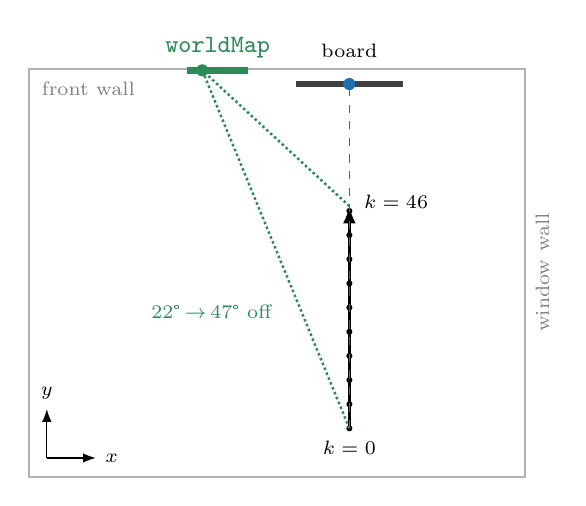
\begin{tikzpicture}[x=0.62cm,y=0.62cm,font=\small]
  % room outline (schematic: floor x -5.67..4.5, back y -4.79, front wall y 3.573)
  \draw[gray!60,line width=0.8pt] (-5.67,-4.79) rectangle (4.5,3.573);
  \node[gray,anchor=north west,font=\scriptsize] at (-5.6,3.5) {front wall};
  \node[gray,rotate=90,font=\scriptsize] at (4.85,-0.6) {window wall};
  % board
  \draw[line width=2.4pt,black!75] (-0.203,3.259) -- (1.997,3.259);
  \node[anchor=south,font=\scriptsize] at (0.897,3.6) {board};
  % map on the wall
  \draw[line width=2.4pt,cSide] (-2.424,3.54) -- (-1.179,3.54);
  \node[anchor=south,font=\scriptsize,cSide] at (-1.8,3.6) {\code{worldMap}};
  % path
  \draw[-{Latex[length=2.2mm]},line width=1.1pt] (0.897,-3.793) -- (0.897,0.759);
  \foreach \k in {0,5,...,45}{\fill ({0.897},{-3.793+\k*0.098957}) circle (1.1pt);}
  \node[anchor=north,font=\scriptsize] at (0.897,-3.85) {$k=0$};
  \node[anchor=west,font=\scriptsize] at (1.0,0.85) {$k=46$};
  % sight lines
  \draw[cTarget,dashed] (0.897,-3.793) -- (0.897,3.259);
  \fill[cTarget] (0.897,3.259) circle (2.2pt);
  \draw[cSide,densely dotted,line width=0.9pt] (0.897,-3.793) -- (-2.116,3.540);
  \draw[cSide,densely dotted,line width=0.9pt] (0.897,0.759) -- (-2.116,3.540);
  \fill[cSide] (-2.116,3.540) circle (2.2pt);
  \node[cSide,font=\scriptsize,anchor=east] at (-0.5,-1.4) {22°\,$\to$\,47° off};
  % axes
  \draw[-{Latex[length=1.6mm]}] (-5.3,-4.4) -- (-4.3,-4.4) node[right,font=\scriptsize] {$x$};
  \draw[-{Latex[length=1.6mm]}] (-5.3,-4.4) -- (-5.3,-3.4) node[above,font=\scriptsize] {$y$};
\end{tikzpicture}
\caption{The Classroom from above, to scale for the walls, board, map and path; the furniture is not drawn. The head walks along $x=0.897$\,m at 1.6\,m height
from $k=0$ to $k=46$. Blue: M1's target, the board centre, 2--6° below the heading. Green: M2's off-axis target on the
\code{worldMap}, 22° left of the heading at $k=0$ and 47° at $k=46$. The windows are on the right-hand wall.}
\label{fig:plan}
\end{figure}

\paragraph{The work, and where it ran.} Each experiment was an issue: Chat designed it, wrote the code and its checks,
and ran it on fov-render's calibration room in its sandbox; Code ran it on the Classroom on the workstation and
reported; Luiz decided whenever a run stopped (Section~\ref{sec:process}). The Classroom is cheap to render this way: the
94 looks of M1 took 19.5\,s, about 0.2\,s a look of which 0.06\,s is rendering\WS.

% ================================================================================================
\section{A preflight along the path}\label{sec:preflight}

fov-render's scene gate checks a scene from its \code{EYE}: holes (rays that leave the scene), back-faces on closed
meshes, and the nearest surface. A head that moves can walk into geometry, or toward a window, that the gate never saw.
So every run starts with a \emph{preflight}: the gate's sanity panorama (720\,px, 4\,spp) from \emph{every} head of the
path, with the scene's limits (clearance 0.25\,m), plus a control head 10\,cm in front of the board, which must fail.
\code{run} refuses to start without it.

\paragraph{The windows.} On the Classroom the preflight failed at 41 of the 47 heads\WS: holes from 0.0250 to 0.0383,
against the scene's limit of 0.025 (fov-render D18, set from the \code{EYE} at $(-0.6,-1.0,1.2)$, where it measured
0.0206). Code's diagnosis\WS: at every head, all of the hole solid angle points at the right-hand wall's window band
(Figure~\ref{fig:holes}). The path runs 1.5\,m nearer that wall and 0.4\,m higher than the \code{EYE}, abeam of the
windows from $k\approx6$ on. The path's own spec had foreseen it. Luiz set this path's limit to 0.046, the measured
maximum plus about a fifth, as D18 had done (M-D6); everything else passed, clearance at least 0.79\,m.

\begin{figure}[t]
\centering
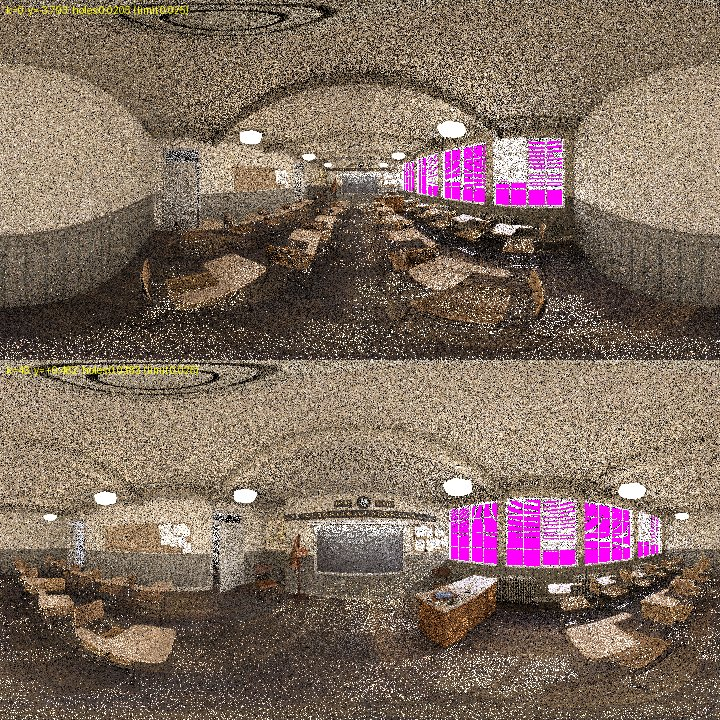
\includegraphics[width=0.48\linewidth]{figs/m1_preflight_holes.jpg}\hfill
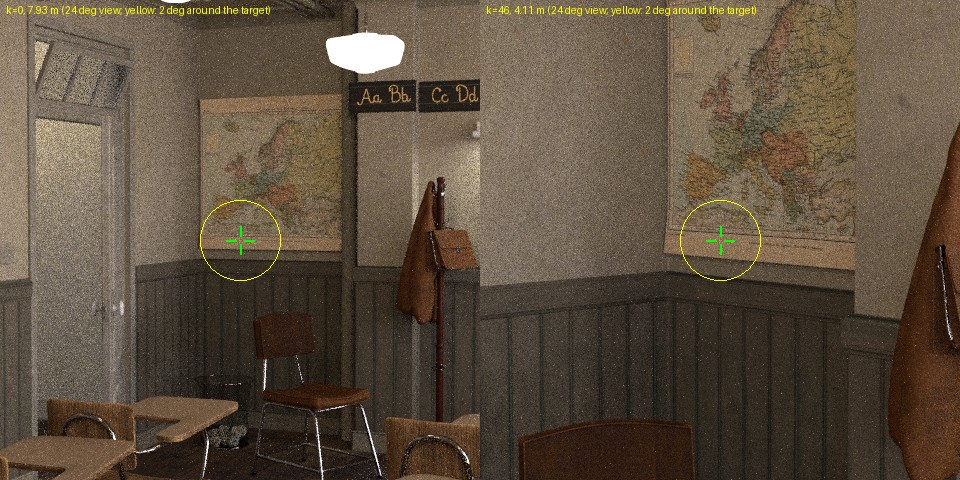
\includegraphics[width=0.48\linewidth]{figs/m2_target_views.jpg}
\caption{Left: the preflight panoramas at $k=0$ and $k=43$, holes in magenta; the centre is the board, the right the
window wall\WS. Right: 24° views toward M2's off-axis target from $k=0$ and $k=46$; green is the target, yellow the 2°
around it\WS.}
\label{fig:holes}
\end{figure}

\paragraph{The target.} M2's off-axis target is given as a ray, not a point: the first opaque surface from the first
head toward the front wall's plane, 2.9\,m left of the board centre, at its height. The preflight finds that surface,
passing through objects the scene's material audit flags as non-opaque (glass, fog), and requires the target to be
visible from every head; its control, a point 0.5\,m behind the target, must be hidden from all of them. In the sandbox
this caught our first choice, a point on the floor, hidden from six heads by a test card\SB. On the Classroom the ray
landed on the \code{worldMap}\WS, a map of Europe hanging on the front wall, a few centimetres proud of it, visible from all
47 heads (Figure~\ref{fig:holes}). The aim had taken the board's plane ($y=3.259$) for the wall's ($y=3.573$); Luiz
accepted the map as the target (M-D8). The fixated point is on the map's bottom roller, so the fovea sees a small depth
step rather than a single plane.

% ================================================================================================
\section{M1: the dolly}\label{sec:m1}

\subsection{Checks}

Each check has a control that must fail. On the Classroom all four passed and every control failed\WS
(Table~\ref{tab:m1}).

\begin{table}[h]
\centering\small
\begin{tabularx}{\linewidth}{@{}lLlL@{}}
\toprule
& what & result\WS & control (must fail) \\
\midrule
M1.0 & every record agrees with its Position pass & p99.9 $\le$ 0.00082°, limit 1.17° & directions turned by 1.5 pixels \\
M1.1 & every record sits on its path head & errors exactly 0 & the path shifted by one step \\
M1.2 & in \code{target} mode the fovea's centre is on the target & within 7.7\,\textmu m (tol.\ 4.4--12.4\,mm) & the target 10\,cm sideways \\
M1.3 & look $k{+}1$'s points reproject onto look $k$'s surface & 0.900--0.990 agree ($\ge 0.80$) & look $k$'s eye 10\,cm sideways: $\le 0.040$ \\
\bottomrule
\end{tabularx}
\caption{M1's checks on the Classroom, both gaze modes. M1.3 counts the points of look $k{+}1$ that land, in look $k$,
on a pixel whose own Position is within 2 pixels at the range; it is lowest at the back of the room, where desks
occlude most.}
\label{tab:m1}
\end{table}

\subsection{Flow}

For the points M1.3 finds in both looks, we measure their retinal displacement between consecutive looks, in degrees and
in raster pixels, against eccentricity (Table~\ref{tab:flow}, Figure~\ref{fig:m1}).

\begin{table}[h]
\centering\small
\begin{tabular}{@{}lccccccc@{}}
\toprule
eccentricity (deg) & 0--1 & 1--2 & 2--5 & 5--10 & 10--20 & 20--30 & 30--45 \\
\midrule
\code{ahead}, deg & 0.013 & 0.031 & 0.072 & 0.151 & 0.312 & 0.606 & 1.066 \\
\code{ahead}, px & 0.20 & 0.35 & 0.52 & 0.64 & 0.75 & 0.94 & 1.16 \\
\code{target} (board), deg & 0.013 & 0.031 & 0.071 & 0.150 & 0.311 & 0.600 & 1.062 \\
\code{target} (board), px & 0.19 & 0.35 & 0.51 & 0.64 & 0.74 & 0.93 & 1.18 \\
\code{target} (map), deg & 0.007 & 0.017 & 0.042 & 0.099 & 0.234 & 0.531 & 0.958 \\
\code{target} (map), px & 0.11 & 0.20 & 0.32 & 0.46 & 0.66 & 1.00 & 1.51 \\
\bottomrule
\end{tabular}
\caption{Median retinal flow per 9.9\,cm step on the Classroom, by eccentricity in the later look\WS.}
\label{tab:flow}
\end{table}

\begin{figure}[t]
\centering
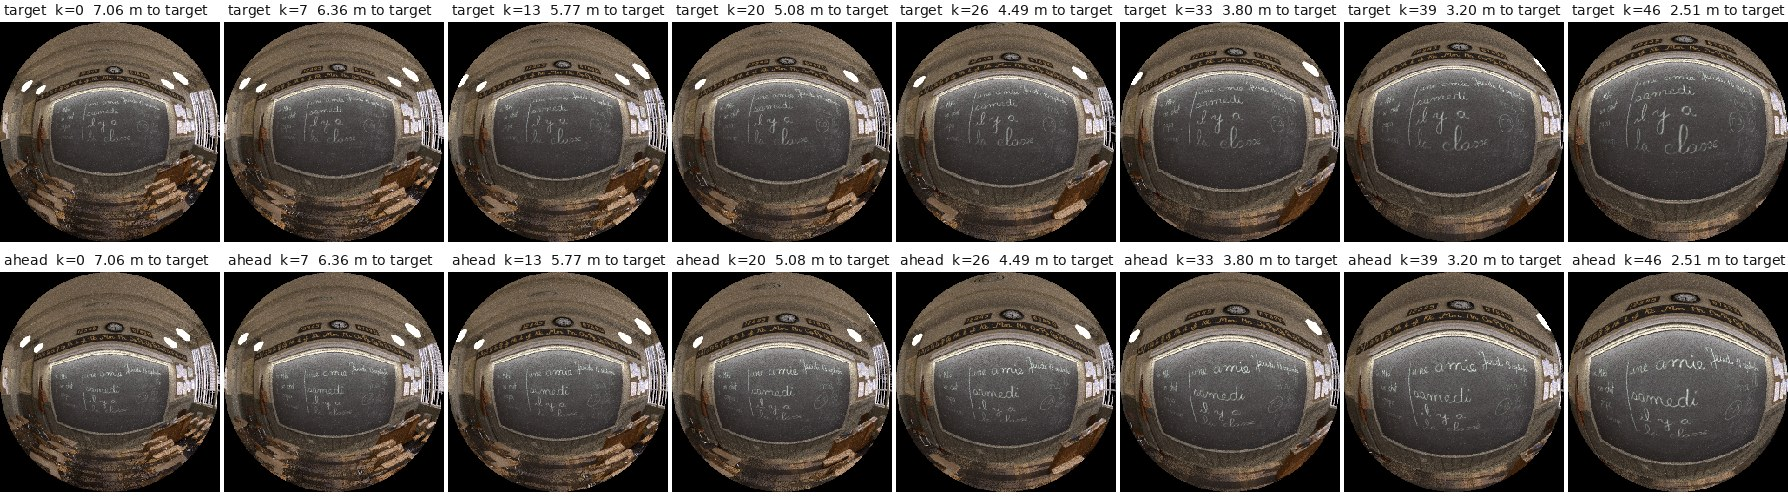
\includegraphics[width=\linewidth]{figs/m1_contact_sheet.jpg}\\[4pt]
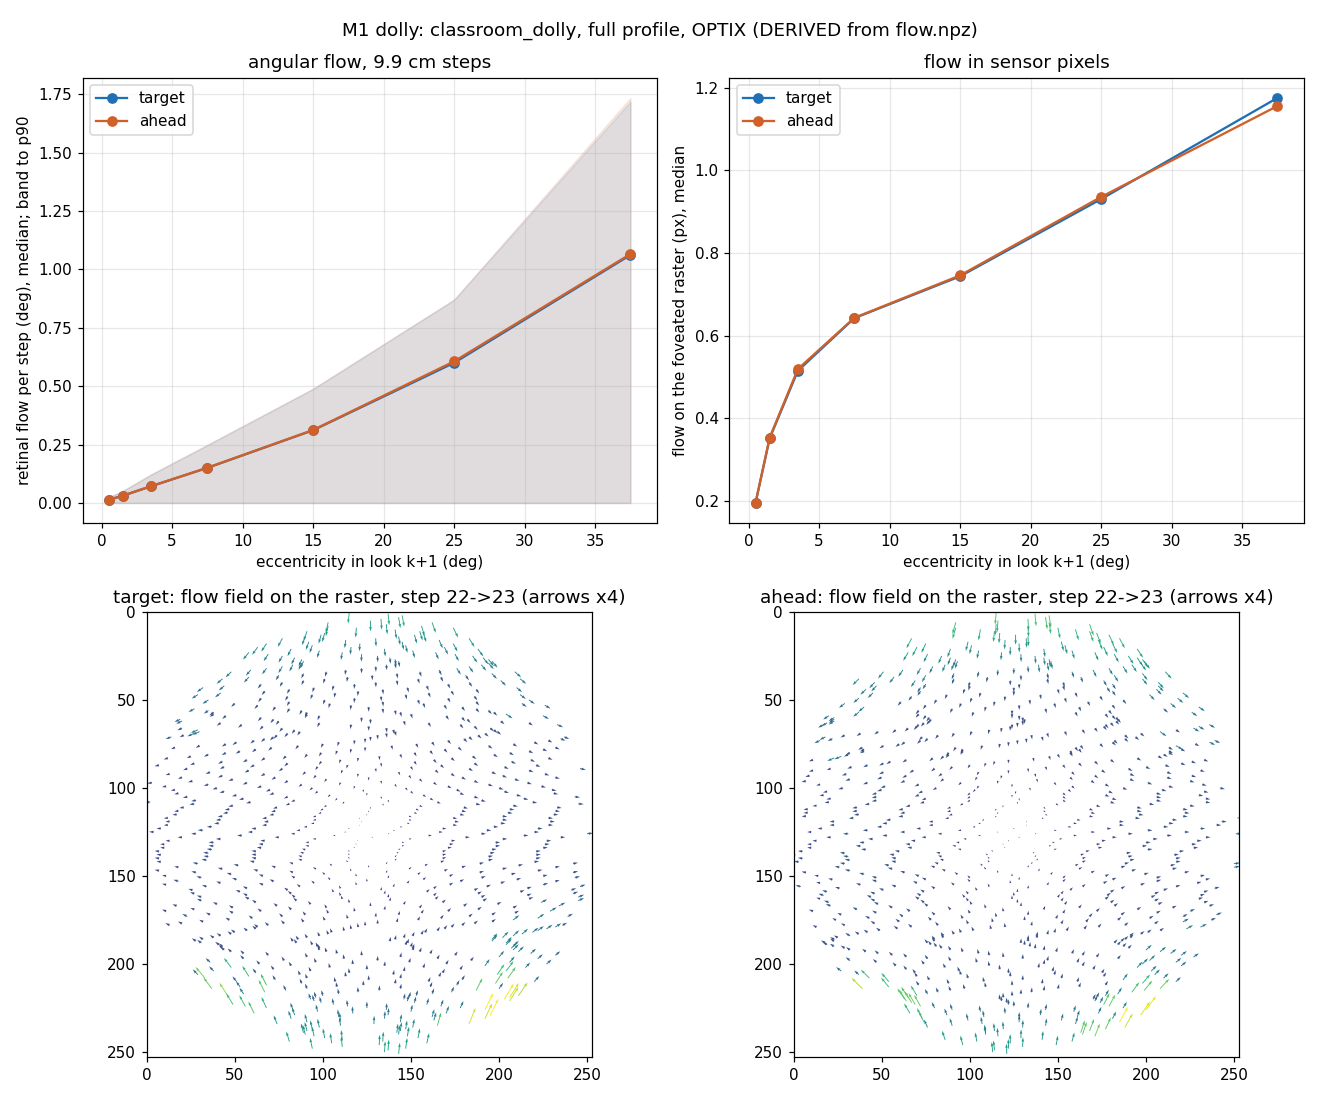
\includegraphics[width=0.82\linewidth]{figs/m1_flow.png}
\caption{M1 on the Classroom\WS. Top: the foveated rasters along the path, fixating the board centre (upper row) and
looking ahead (lower row); the log-polar image gives most of its pixels to the fovea, at the centre. Bottom: the flow
per step against eccentricity, in degrees and in raster pixels, and the flow field of the middle step on the raster
(arrows $\times4$).}
\label{fig:m1}
\end{figure}

\paragraph{Fixating the board changes nothing in the medians.} The two modes agree within 0.01°. This is expected for this
target. The eye turns only 0.03° per step at the back of the room and 0.24° at the front to hold the board centre. For a
plane facing the head, a translation together with the rotation that holds one of its points still is, to first order,
an expansion about that point, at the same rate as the expansion about the focus of expansion when looking ahead. The
board fills the fovea and most of the field, so the medians match. Only points off the board's plane separate the modes,
by a parallax proportional to the 2--6° between target and heading. In \code{target} mode the focus of expansion sits
29--56 raster pixels above the fovea. The off-axis target of M2 does separate them: its flow is about half as large in
the fovea, where the fixated map is.

\paragraph{The raster flow is not flat.} In degrees the flow grows with eccentricity, as Eq.~\eqref{eq:flow} says. On a
log-polar raster the pixel grows as $(E_2+e)$, so the flow in pixels is flat only where the range is about the same in
every direction. In both rooms the periphery sees nearer surfaces (floor, ceiling, desks) than the centre, and the flow
in pixels rises from about 0.6 at 5--10° to 1.2 at 30--45° looking ahead\WS. The calibration room rises by
the same factor, $\times1.7$ against $\times1.8$\SB. Its pixel values are half the Classroom's only because the sandbox
used the \code{small} raster ($s_0=0.1^\circ$); in degrees the two rooms agree within about 10\,\% at 30--45°. Our first
reading of the sandbox, ``nearly flat'', was true of its \code{target} mode only, and was corrected when the Classroom
numbers came in. A flat radial flow on a log-polar raster under approach to a surface is the classic result of
Tistarelli and Sandini~\cite{tistarelli}; a cluttered room is not that surface.

% ================================================================================================
\section{M2: range from the head's motion}\label{sec:m2}

\subsection{Method}

The head's step between two looks is known (the path), and so are the eye's poses (the records). Two looks of a point
therefore give its range by triangulation, with the path segment as the baseline, like stereo with the eyes one behind
the other. For each pair of looks $(a, b{=}a{+}s)$, with strides $s=1,5,10$ (0.10, 0.49, 0.99\,m), and each surface
sample of look $b$:
\begin{itemize}
\item \textbf{Correspondence} by the oracle, as in M1.3: where $b$'s point $P$ projects in look $a$, and whether $a$ sees
  it there. Occluded points have no match.
\item \textbf{Pixel-limited range}: the ray through $b$'s pixel centre, $\vb c_b+t\,\vb d_b$, and the ray through the
  centre of the pixel of $a$ that $P$ projects to, $\vb c_a+u\,\vb d_a$, are triangulated by their closest points:
  \begin{equation}\label{eq:tri}
    \hat\rho = t^\ast = \frac{\vb d_b\!\cdot\!\vb w - \beta\,\vb d_a\!\cdot\!\vb w}{1-\beta^2},\qquad
    \vb w = \vb c_a-\vb c_b,\quad \beta = \vb d_a\!\cdot\!\vb d_b .
  \end{equation}
  If the rays are parallel there is no range.
\item \textbf{Truth}: $\rho=|P-\vb c_b|$ from $b$'s Position pass. A range is \emph{usable} when it is within 10\,\% (a
  reporting threshold, not a pass/fail).
\item \textbf{Bracket}: the ranges along $b$'s ray whose projection into $a$ stays inside the matched pixel, as a relative
  half-width; that is, the precision the match supports, whatever its error turned out to be (Section~\ref{sec:samepixel}).
\item \textbf{Model}: rounding $a$'s pixel only (b's sample is its own pixel's centre, and its Position, the pixel's mean,
  lies on that ray to first order),
  \begin{equation}\label{eq:model}
    \frac{\delta\rho}{\rho} \approx \frac{\rho\,\sigma}{|T|\sin\psi},\qquad \sigma=\sqrt{\omega_a/12},
  \end{equation}
  with $\omega_a$ the pixel's solid angle and $\psi$ the angle between $b$'s ray and the baseline. For rounding alone the
  median $|$error$|$ is $\sqrt3/2\approx0.87$ times the model.
\end{itemize}
Check M2.1: with the exact rays through $P$, Eq.~\eqref{eq:tri} returns the true range (relative error at most
$10^{-6}$ where the rays are at least 0.01° apart); its control moves $a$'s eye centre 1\,cm along the path and must
give a median error of at least $10^{-3}$. It passed on all runs, maximum error $2.8\times10^{-8}$, and the control
failed with a median of 0.101\WS.

\subsection{Results}

Table~\ref{tab:m2} gives the fovea ($e<2^\circ$) for the three gaze conditions on the Classroom; Figure~\ref{fig:m2sum} gives
the bracket across the field, and Figure~\ref{fig:m2} the full depth figures.

\begin{table}[h]
\centering\footnotesize\setlength{\tabcolsep}{4.5pt}
\begin{tabular}{@{}llcccc@{}}
\toprule
gaze & stride & error: median \textbar{} usable & bracket: median \textbar{} usable & same pixel & field, by bracket \\
\midrule
\multirow{3}{*}{\code{ahead}} & 0.10\,m & no range \textbar{} 0.00 & no range \textbar{} 0.00 & 0.92 & 0.000 \\
 & 0.49\,m & 0.164 \textbar{} 0.31 & 0.463 \textbar{} 0.00 & 0.05 & 0.101 \\
 & 0.99\,m & 0.094 \textbar{} 0.53 & 0.213 \textbar{} 0.00 & 0.01 & 0.612 \\
\midrule
\multirow{3}{*}{\shortstack[l]{\code{target}, board\\ 2--6° off}} & 0.10\,m & 0.201 \textbar{} 0.26 & 0.549 \textbar{} 0.00 & 0.93 & 0.001 \\
 & 0.49\,m & 0.046 \textbar{} 0.81 & 0.112 \textbar{} 0.43 & 0.05 & 0.244 \\
 & 0.99\,m & 0.026 \textbar{} 0.96 & 0.061 \textbar{} 0.84 & 0.01 & 0.730 \\
\midrule
\multirow{3}{*}{\shortstack[l]{\code{target}, map\\ 22--47° off}} & 0.10\,m & 0.010 \textbar{} 0.996 & 0.073 \textbar{} 0.75 & 1.00 & 0.167 \\
 & 0.49\,m & 0.008 \textbar{} 0.992 & 0.015 \textbar{} 0.99 & 0.21 & 0.829 \\
 & 0.99\,m & 0.004 \textbar{} 0.995 & 0.008 \textbar{} 0.995 & 0.05 & 0.851 \\
\bottomrule
\end{tabular}
\caption{M2 on the Classroom\WS: the fovea ($e<2^\circ$). ``Usable'' is the fraction of all the fovea's samples within 10\,\%;
``same pixel'' the fraction of matches that land on the same raster pixel in both looks; the last column is the whole
field's fraction usable by bracket.}
\label{tab:m2}
\end{table}

\begin{figure}[t]
\centering
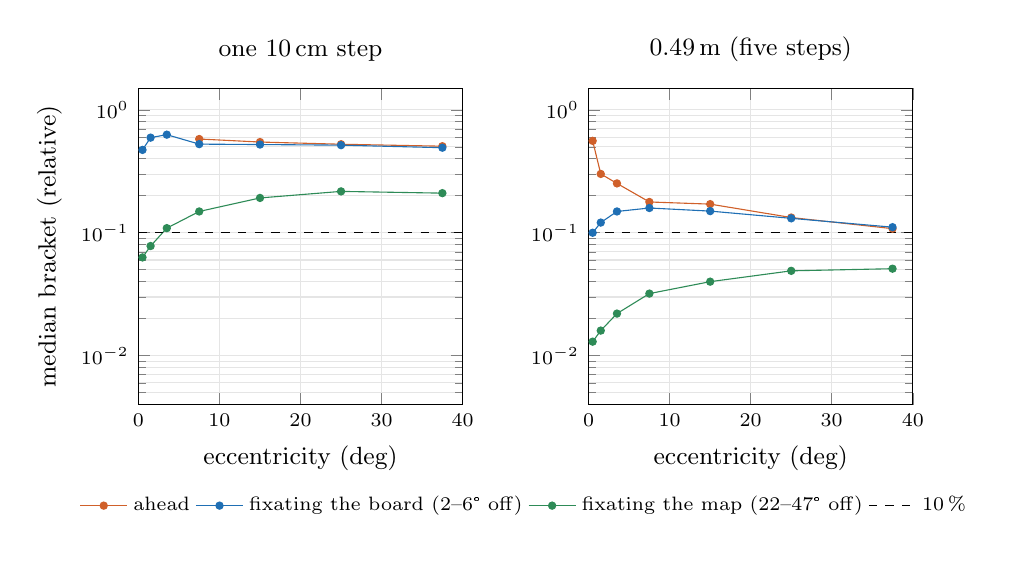
\begin{tikzpicture}
\begin{groupplot}[group style={group size=2 by 1, horizontal sep=1.6cm},
  width=0.47\linewidth, height=5.6cm, ymode=log, xmin=0, xmax=40,
  xlabel={eccentricity (deg)}, grid=both, grid style={gray!20},
  legend style={font=\scriptsize, legend columns=4, draw=none}, tick label style={font=\scriptsize},
  label style={font=\small}, title style={font=\small}]
\nextgroupplot[title={one 10\,cm step}, ylabel={median bracket (relative)}, ymin=0.004, ymax=1.5,
    legend to name=m2leg]
  \addplot[cAhead, mark=*, mark size=1.3pt] coordinates {(7.5,0.579) (15,0.547) (25,0.525) (37.5,0.506)};
  \addplot[cTarget, mark=*, mark size=1.3pt] coordinates {(0.5,0.472) (1.5,0.594) (3.5,0.628) (7.5,0.526) (15,0.522) (25,0.516) (37.5,0.492)};
  \addplot[cSide, mark=*, mark size=1.3pt] coordinates {(0.5,0.063) (1.5,0.078) (3.5,0.109) (7.5,0.149) (15,0.192) (25,0.217) (37.5,0.210)};
  \addplot[black, dashed, domain=0:40] {0.1};
  \legend{ahead, fixating the board (2--6° off), fixating the map (22--47° off), 10\,\%}
\nextgroupplot[title={0.49\,m (five steps)}, ymin=0.004, ymax=1.5]
  \addplot[cAhead, mark=*, mark size=1.3pt] coordinates {(0.5,0.559) (1.5,0.301) (3.5,0.252) (7.5,0.178) (15,0.171) (25,0.133) (37.5,0.108)};
  \addplot[cTarget, mark=*, mark size=1.3pt] coordinates {(0.5,0.100) (1.5,0.121) (3.5,0.149) (7.5,0.159) (15,0.150) (25,0.131) (37.5,0.111)};
  \addplot[cSide, mark=*, mark size=1.3pt] coordinates {(0.5,0.013) (1.5,0.016) (3.5,0.022) (7.5,0.032) (15,0.040) (25,0.049) (37.5,0.051)};
  \addplot[black, dashed, domain=0:40] {0.1};
\end{groupplot}
\node[below=0.9cm] at ($(group c1r1.south)!0.5!(group c2r1.south)$) {\pgfplotslegendfromname{m2leg}};
\end{tikzpicture}
\caption{The precision a match supports, across the field, on the Classroom\WS: the median bracket by eccentricity
(bin centres; dashed: 10\,\%). Looking ahead, a 10\,cm step gives no range at all within 5° (not plotted). Fixating far off
the heading, the fovea is the most precise part of the field, and the precision falls with eccentricity as the pixels
grow; fixating near the heading, or looking ahead, the fovea is among the worst.}
\label{fig:m2sum}
\end{figure}

\begin{figure}[t]
\centering
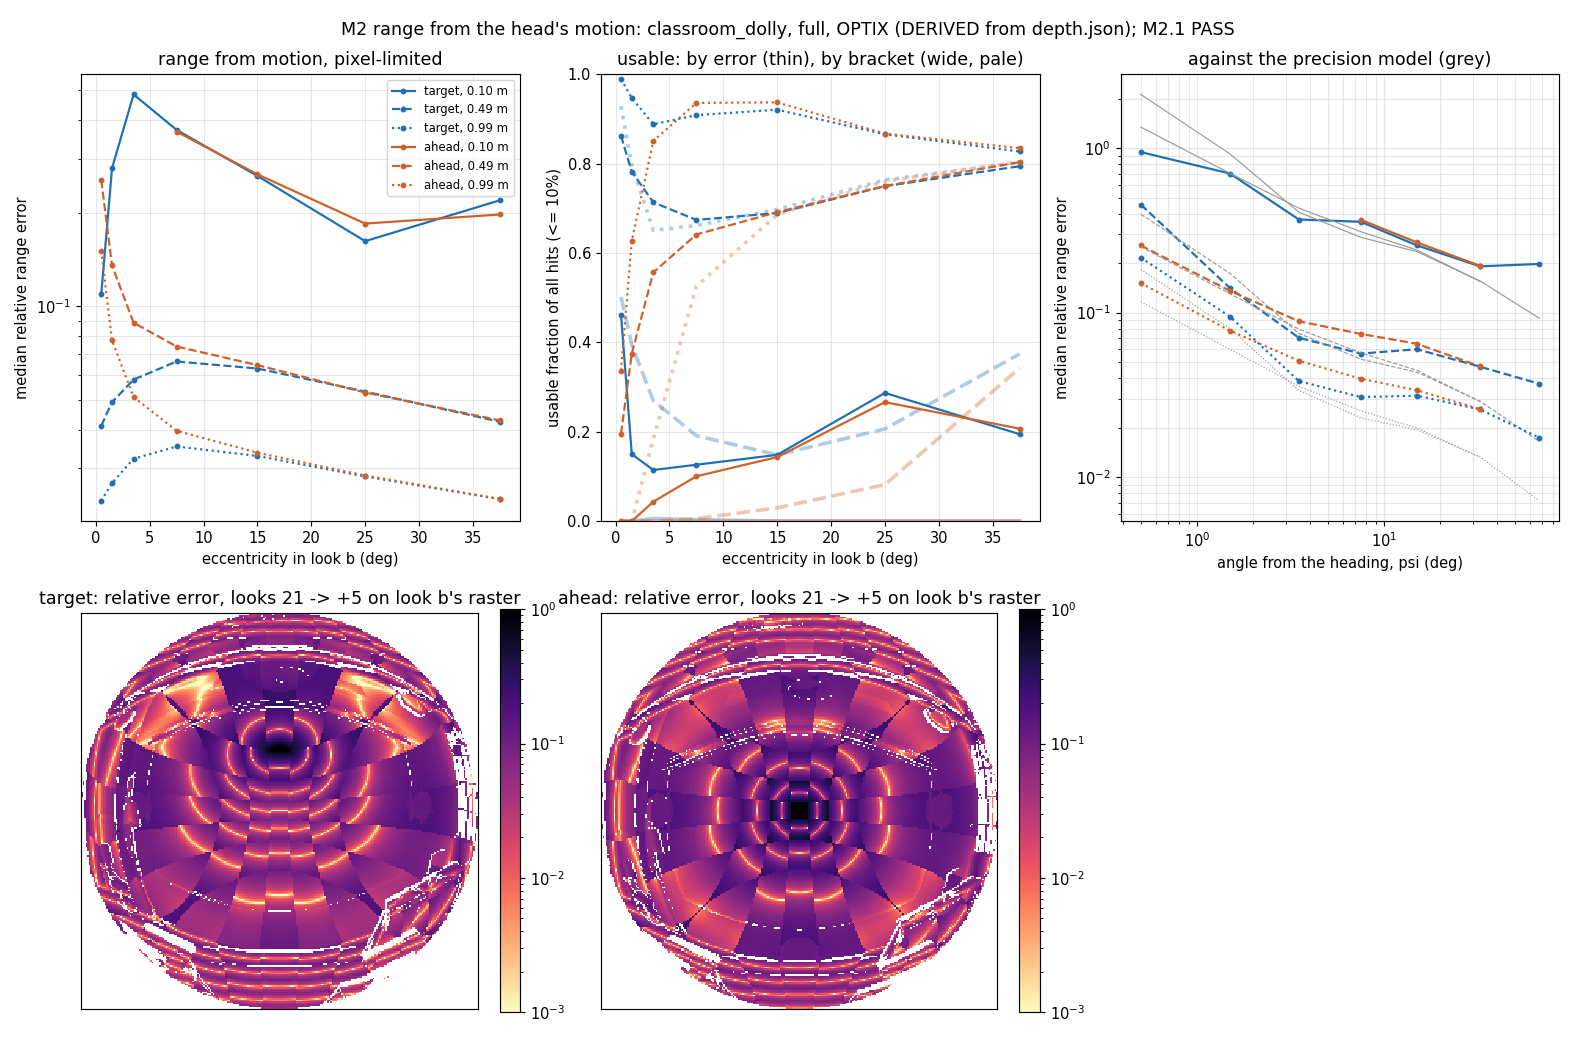
\includegraphics[width=0.92\linewidth]{figs/m2_depth_dolly1.png}\\[6pt]
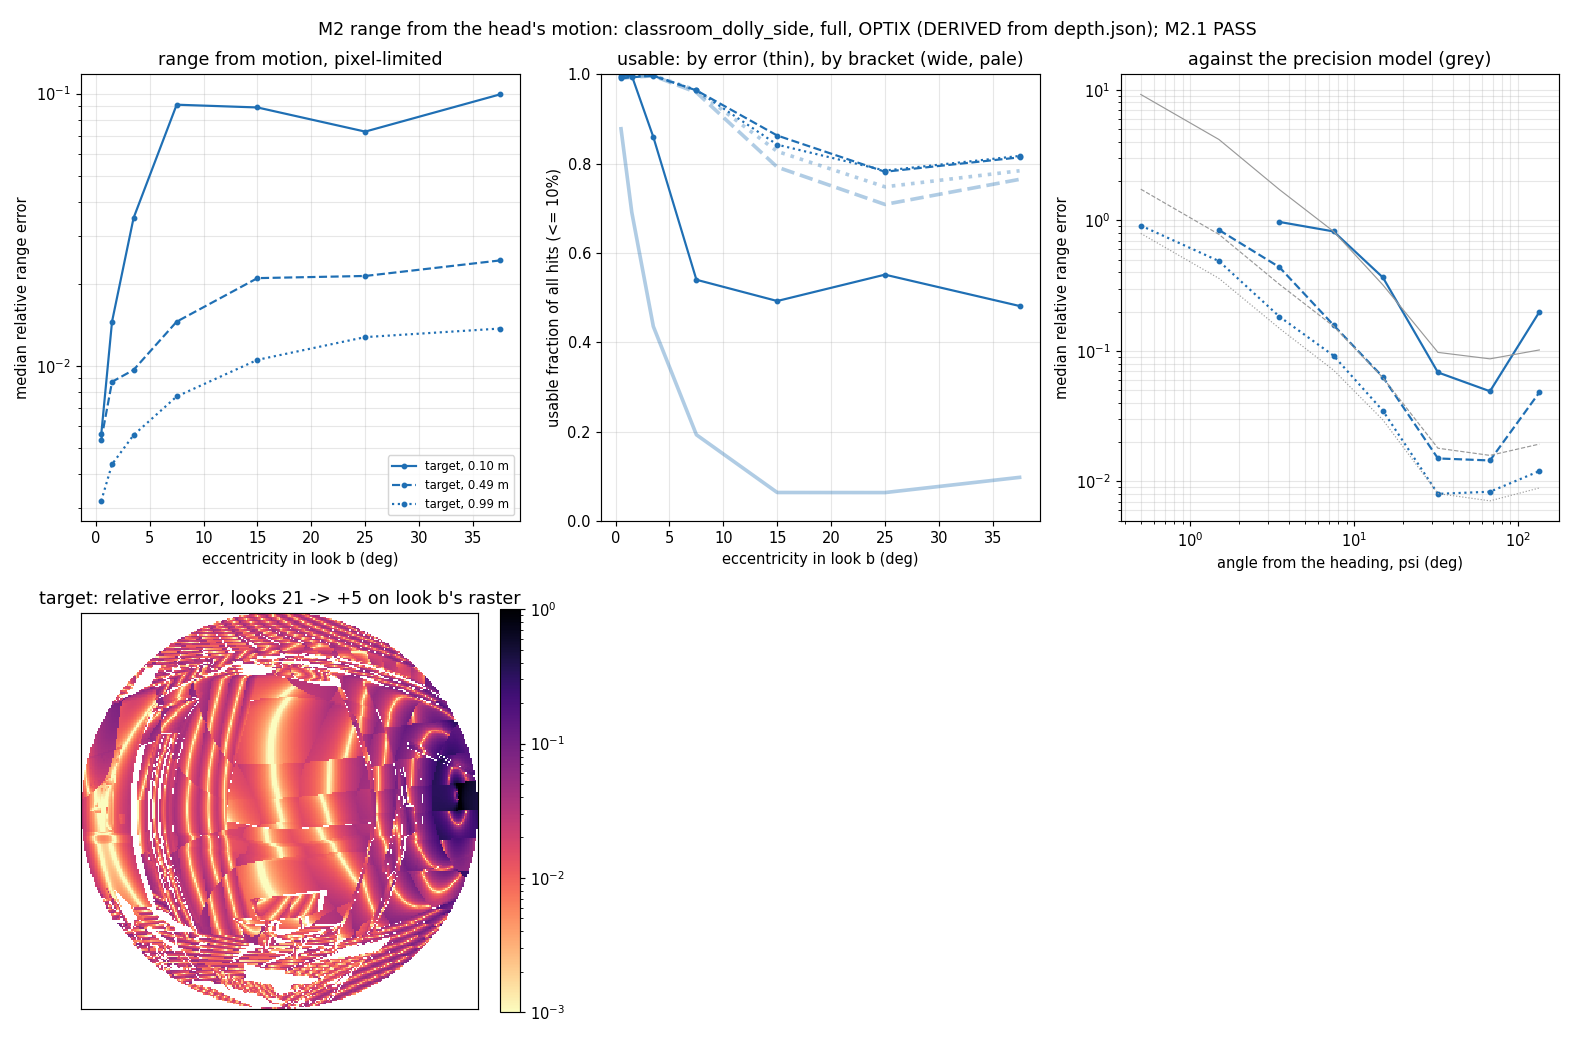
\includegraphics[width=0.92\linewidth]{figs/m2_depth_side.png}
\caption{M2's depth figures on the Classroom\WS, top the M1 run (both modes), bottom the off-axis run. In each: the median
error and the usable fraction by eccentricity (thin: by error; wide, pale: by bracket), the error against the angle from
the heading with the model of Eq.~\eqref{eq:model} in grey, and the error on the raster for the middle pair at 0.49\,m.}
\label{fig:m2}
\end{figure}

\paragraph{Where the eye looks decides what the fovea can range.} Looking along the path, the fovea gets no usable range
at any stride: none at all from one step, and a bracket of 21\,\% from 1\,m. Its finest pixels sit where $\sin\psi$ in
Eq.~\eqref{eq:model} vanishes. Fixating a point 22--47° off the heading puts them where the parallax is: the fovea then
supports 7.3\,\% from a single 10\,cm step (three quarters of its samples within 10\,\%), 1.5\,\% from 0.49\,m and
0.8\,\% from 0.99\,m, and becomes the most precise part of the field (Figure~\ref{fig:m2sum}). Fixating the board, only
2--6° off the heading, is in between: nothing usable from one step, 6.1\,\% from 1\,m. The calibration room gave the
same picture\SB: off the path's line 8.9, 1.9 and 1.0\,\%; looking ahead nothing usable at any stride.

\paragraph{Errors outgrow rounding at longer strides.} The median error over the model of Eq.~\eqref{eq:model} rises with
the stride on the M1 run, from 1.07--1.11 at 0.10\,m to 1.41--1.48 at 0.49\,m and 1.68--1.75 at 0.99\,m\WS (0.87 is
rounding alone); the sandbox gave 1.0--1.7\SB. Depth edges and the pixel-mean Position at them, curved surfaces within a
pixel, and the model's linearisation in $\psi$ are the likely causes; we have not separated them.

\subsection{Same pixel, and why we report a bracket}\label{sec:samepixel}

Our first version of M2 reported only the error, and it read the off-axis fovea as giving 1--3\,\% from one step. Code
found the catch\WS: at a 10\,cm step \emph{every} foveal match of the off-axis run lands on the same raster pixel in both
looks; its flow is under half a pixel. The code then said such a match gives no range, which is true only when the eye
does not turn. Under fixation the rays through one pixel from the two eye centres are not parallel; they cross on the
surface of zero flow through the fixated point, and that is the range Eq.~\eqref{eq:tri} returned.

That range is legitimate. A same-pixel match is a measurement: the flow is under half a pixel. To first order, it says
\begin{equation}\label{eq:interval}
  \Bigl|\,\frac{1}{\rho}-\frac{1}{\rho_0}\Bigr| \lesssim \frac{p}{2\,|T|\sin\psi},
\end{equation}
an interval in inverse range of the same width with or without rotation ($p$ is the pixel's angular size). Looking ahead
it is centred on $1/\rho_0=0$, so it bounds the range from below only: no range. Fixating, it is centred on the zero-flow
surface, so it bounds the range on both sides. This is the active-vision argument that fixation makes depth well posed,
relative to the fixated point~\cite{aloimonos,ballard}. What the error alone could not show is how much that measurement
supports. On the off-axis run the map lies close to the zero-flow surface, so its points sit near the pixels' centres
and the error came out below what rounding allows (error over model 0.75 at 10\,cm\WS, against 0.87). That is the
geometry's luck, not the sensor's precision. The bracket reports the precision; it is 7.3\,\% where the error was
1.0\,\%. Adding the bracket changed none of the error-based numbers: Code compared all 1{,}210 values of the Classroom
records before and after, and the sandbox's 882\SB, and found no difference.

% ================================================================================================
\section{How the work was done}\label{sec:process}

The method is the N-Surface method~\cite{nsurface} in its lighter form from fov-render: one file of rules
(\code{CLAUDE.md}) and GitHub issues as the channel between Claude in a chat sandbox (``Chat''), which plans, writes the
code and its checks and runs what a CPU can, and Claude Code on the workstation (``Code''), which runs what needs the
GPU or the Classroom files and reports; Luiz decides and accepts. Every number says where it was measured; every check
ships a control that must fail; nothing changes a threshold to make something pass. Issue~\#1 was M1, issue~\#3 M2,
each closed by a pull request.

The record of this phase is mostly a record of stops and corrections, and that is how it should read:
\begin{itemize}
\item Two runs stopped at the preflight, as their issues said they should: once on the windows (M-D6), once on a target
  that was a map, not a wall (M-D8). Neither was fixed by the agent that found it; both went to Luiz with options.
\item Two readings were corrected. Chat's ``the raster flow is nearly flat'' did not survive the Classroom
  (Section~\ref{sec:m1}). Chat's ``1--3\,\% from one step'' did not survive Code's same-pixel analysis
  (Section~\ref{sec:samepixel}); the fix kept every earlier number and added the bracket.
\item Code confirmed the sandbox bit for bit on a second machine, and found two smaller faults: the model counted rounding
  in both looks, and the depth records named the commit that rendered the run, not the code that computed them. Both are
  fixed.
\end{itemize}
Luiz also changed one rule along the way: Chat may now edit \code{CLAUDE.md}, in this repository and in fov-render, with
his approval.

% ================================================================================================
\section{Limitations}\label{sec:limits}

\begin{itemize}
\item \textbf{Oracle correspondence.} The renderer says which pixel of one look sees the point of the other. No image
  content is used: M2 measures what the geometry and the raster allow, not what a matcher would achieve.
\item \textbf{Whole-pixel matches.} The match is rounded to a pixel; a real matcher interpolates. Our precision is
  pessimistic by the factor a sub-pixel matcher would gain.
\item \textbf{One path, one off-axis target.} A straight, level walk; the off-axis target is a near-planar map close to
  the zero-flow surface, which flatters the error (not the bracket). Other targets, turns, and paths are untested.
\item \textbf{Monocular, static.} One eye at the cyclopean point; no binocular stereo combined with motion; a static
  scene; motion between looks only.
\item \textbf{The scene.} The Classroom's windows open onto a featureless world (holes up to 3.8\,\% of the sphere on this
  path), and the room is one synthetic interior.
\end{itemize}

\section{Next steps (proposed)}\label{sec:next}

\begin{itemize}
\item \textbf{A gaze policy for depth.} Eq.~\eqref{eq:model} and the bracket predict, before looking, how much range a
  fixation will give along a planned motion. An eye that chooses targets to maximise it is the natural next experiment.
\item \textbf{Accumulate over looks.} Fuse each point's brackets across strides and looks, in inverse range, instead of
  judging pairs.
\item \textbf{Real correspondence.} Replace the oracle with a matcher on the rendered images, sub-pixel, and compare with
  the bracket.
\item \textbf{Two eyes and a moving head.} Combine the playground's binocular stereo with translational parallax, and
  turns of the head (fov-render's head pose already allows them).
\end{itemize}

\paragraph{Records.} Everything above is in \code{visgraf/foveal-motion}~\cite{fm}: \code{docs/motion.md} (the
decisions and all results), \code{docs/runs/issue-1/} and \code{docs/runs/issue-3/} (run records, checks, depth
summaries, the diagnostic scripts), \code{paths/} (the path specs with their sources), and issues \#1 and \#3. The
commands are in the repository's README. On the workstation the looks of both Classroom runs render in about 30\,s and
each preflight takes under a minute\WS; the calibration-room sandbox runs end to end in under a minute on a CPU\SB.

% ================================================================================================
\begin{thebibliography}{99}
\bibitem{fm} VISGRAF Lab. \emph{foveal-motion}: active foveal vision under head motion.
  \url{https://github.com/visgraf/foveal-motion}
\bibitem{fovrender} VISGRAF Lab. \emph{fov-render}: Blender Cycles rendering for gaze-directed binocular observers.
  \url{https://github.com/visgraf/fov-render}
\bibitem{fovrendertr} Luiz Velho and Claude. ``Foveated Stereo Rendering in Blender: A Unified Sensor Framework''.
  Technical Report TR-14-2026, VISGRAF Lab -- IMPA, 2026.
\bibitem{playground} VISGRAF Lab. \emph{foveal-playground}: a playground for active foveal 3-D vision.
  \url{https://github.com/visgraf/foveal-playground}
\bibitem{tr11} Luiz Velho and Claude. ``Active Foveal 3-D Vision Playground''. Technical Report TR-11-2026, VISGRAF
  Lab -- IMPA, 2026.
\bibitem{yarbus} VISGRAF Lab. \emph{yarbus-agent}: question-dependent scanpaths in the Classroom, \code{REPORT.md}.
  \url{https://github.com/visgraf/yarbus-agent}
\bibitem{nsurface} Luiz Velho and Claude. ``The N-Surface Method: Rigor and Spontaneity in Human--AI Research''.
  VISGRAF technical note, 2026.
\bibitem{lhp} H.~C. Longuet-Higgins and K.~Prazdny. The interpretation of a moving retinal image.
  \emph{Proceedings of the Royal Society of London B}, 208:385--397, 1980.
\bibitem{schwartz} E.~L. Schwartz. Spatial mapping in the primate sensory projection: analytic structure and relevance
  to perception. \emph{Biological Cybernetics}, 25:181--194, 1977.
\bibitem{tistarelli} M.~Tistarelli and G.~Sandini. On the advantages of polar and log-polar mapping for direct estimation
  of time-to-impact from optical flow. \emph{IEEE Transactions on Pattern Analysis and Machine Intelligence},
  15(4):401--410, 1993.
\bibitem{aloimonos} J.~Aloimonos, I.~Weiss and A.~Bandyopadhyay. Active vision. \emph{International Journal of Computer
  Vision}, 1(4):333--356, 1988.
\bibitem{ballard} D.~H. Ballard. Animate vision. \emph{Artificial Intelligence}, 48:57--86, 1991.
\end{thebibliography}

\end{document}
